
Shiny is an open source R package that provides an elegant and powerful web framework for building web applications using R \cite{beeley2013}. The ‘app’ can be interacted with by entering data, running functions with user-specified settings to plot figures, and downloading the resultant figures in a variety of formats.

The \texttt{RMDitemfit} Shiny app generates a sampling distribution for different Rasch item fit statistics and visualizes empirical critical values. The app is available free-of-charge (\url{https://shiny.sund.ku.dk/RMDitemfit/}) and can also be found through the \texttt{RASCHplot} package such that users can run the app locally using \texttt{RASCHplot::app("RMDitemfit")}. The graphical user interface of \texttt{RMDitemfit} is displayed in \autoref{fig:userinterface}. 

\begin{figure}[]
\centering
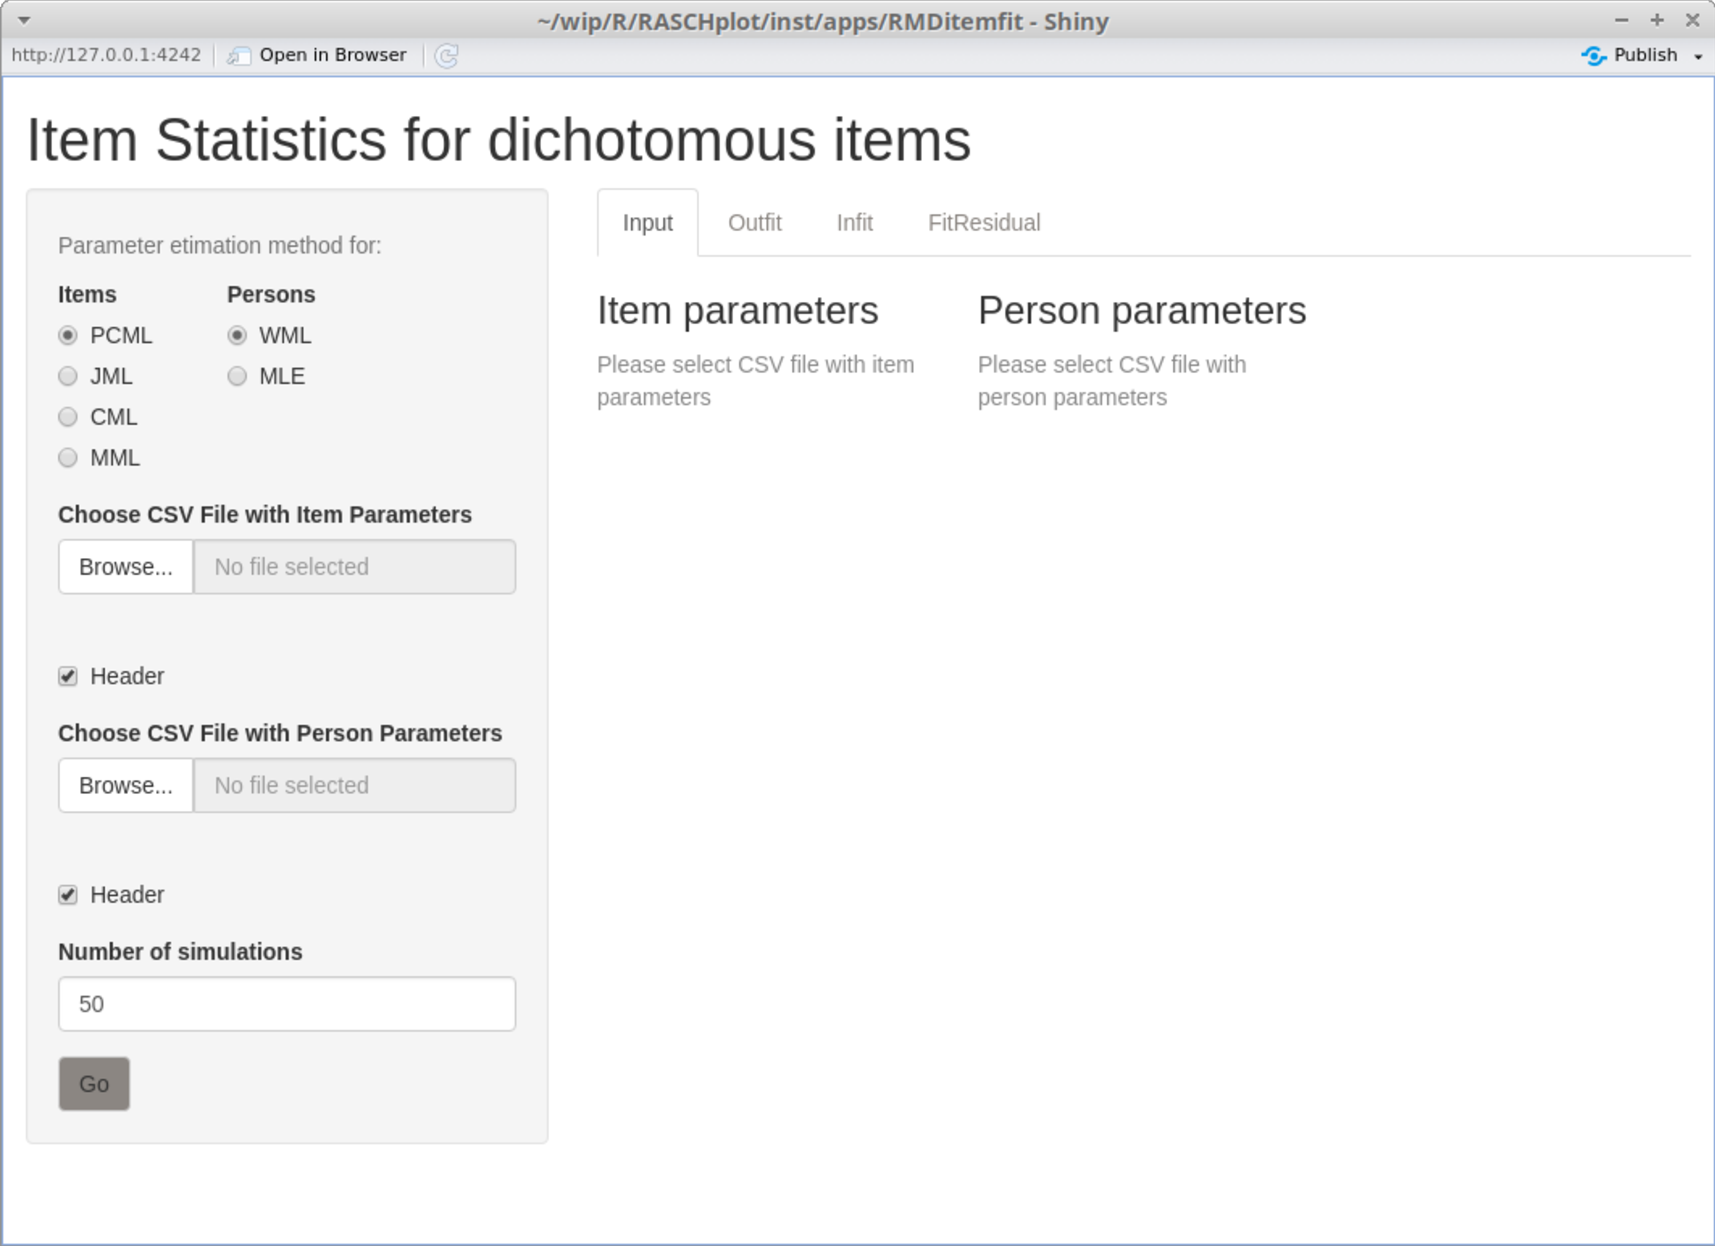
\includegraphics[width = .8\textwidth]{interface}
\caption{Screenshot of the \texttt{RMDitemfit} Shiny app graphical user interface.}
\label{fig:userinterface}
\end{figure}

The sidebar panel contains input controls to select parameter estimation methods, input data, and specify the number of simulations to run. This application requires a vector of item difficulties and a vector of person parameters in two separate files. Users enter their data by uploading CSV files. Once files are uploaded, the data used going forward are shown on the app landing page (the ‘Input’ tab), see \autoref{fig:inputtab}.

Subsequently, when the number of simulations is selected, users proceed to press the `Go` button to see the resultant figures. On the `Outfit` (see \autoref{fig:outfittab}), `Infit`, and `FitResid` tabs the sample distributions for the minimum and maximum outfit, infit, and item fit residuals, respectively, are shown.


\begin{figure}
    \centering
    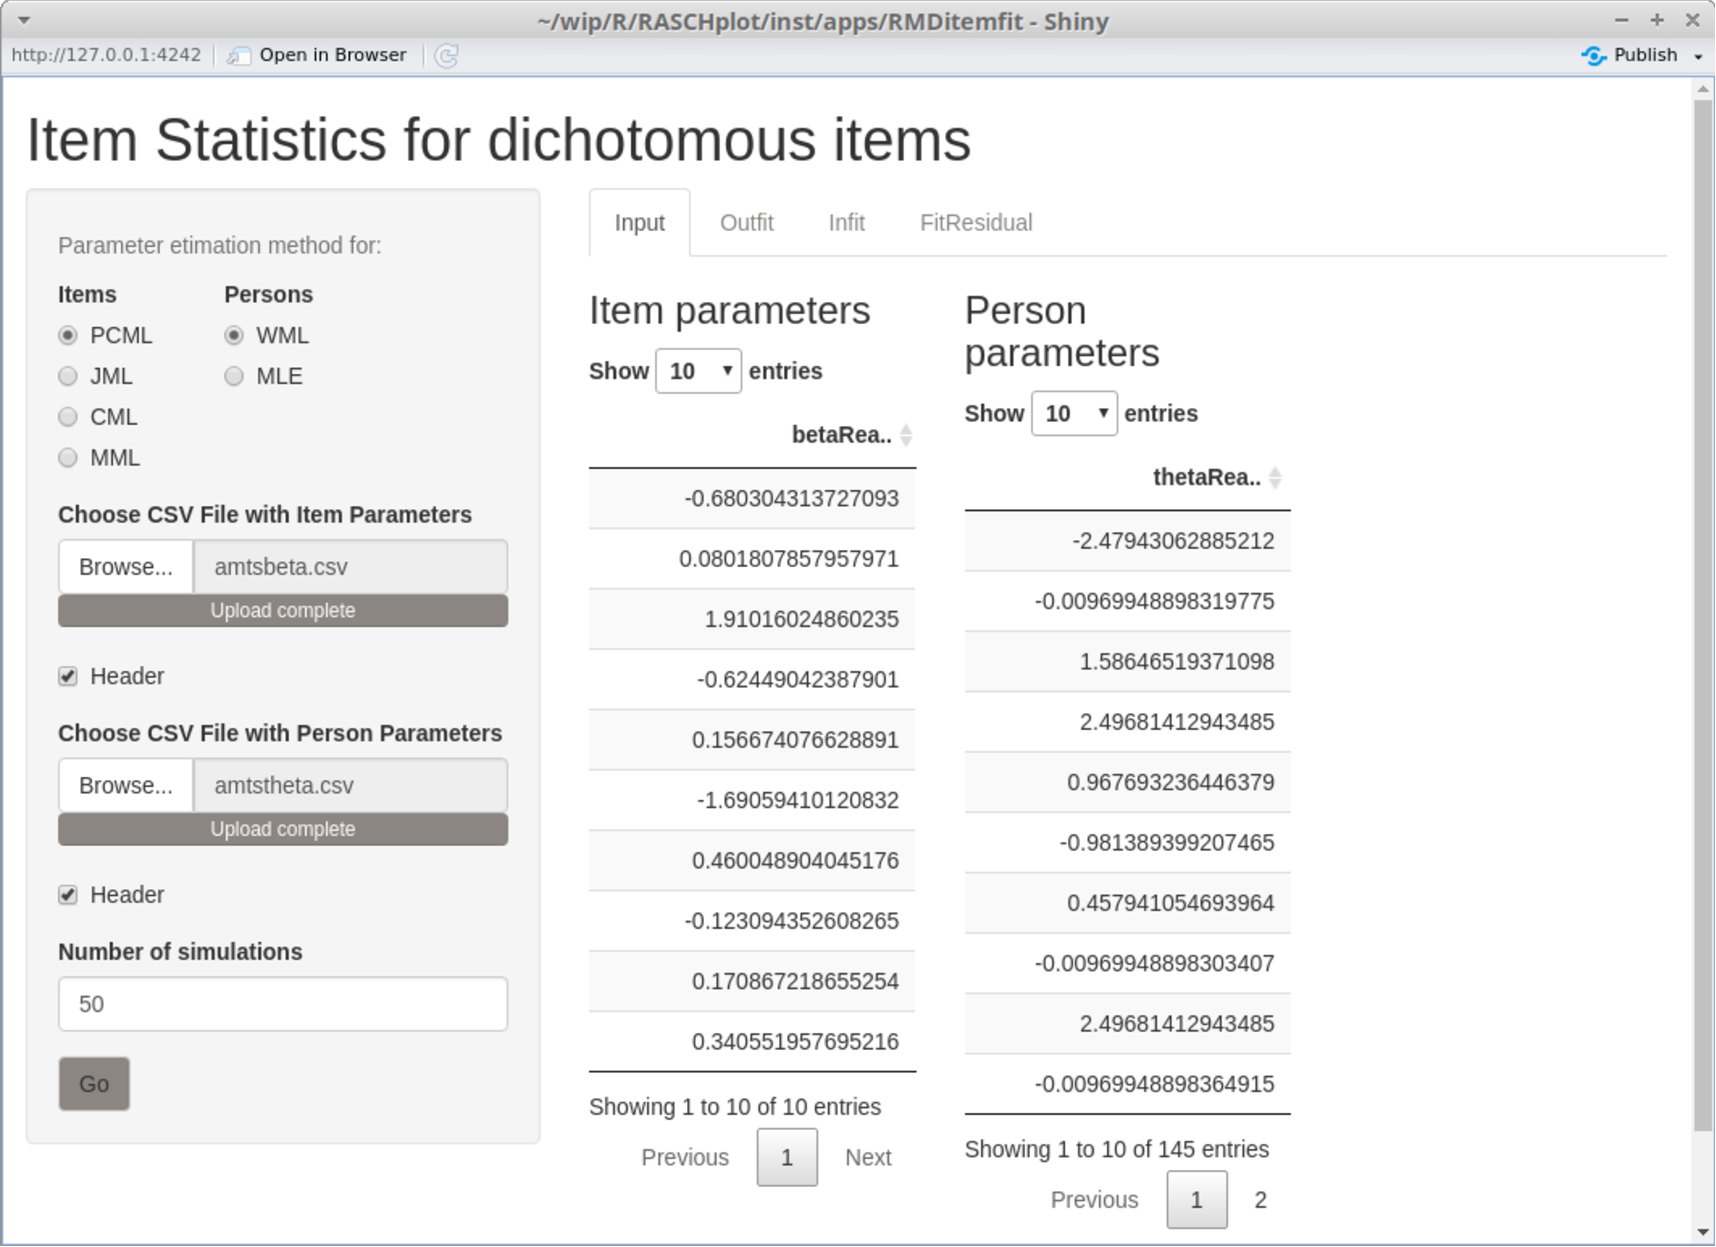
\includegraphics[width = .8\textwidth]{inputtab}
    \caption{Screenshot of the data entry page.}
    \label{fig:inputtab}
\end{figure}

\begin{figure}
    \centering
    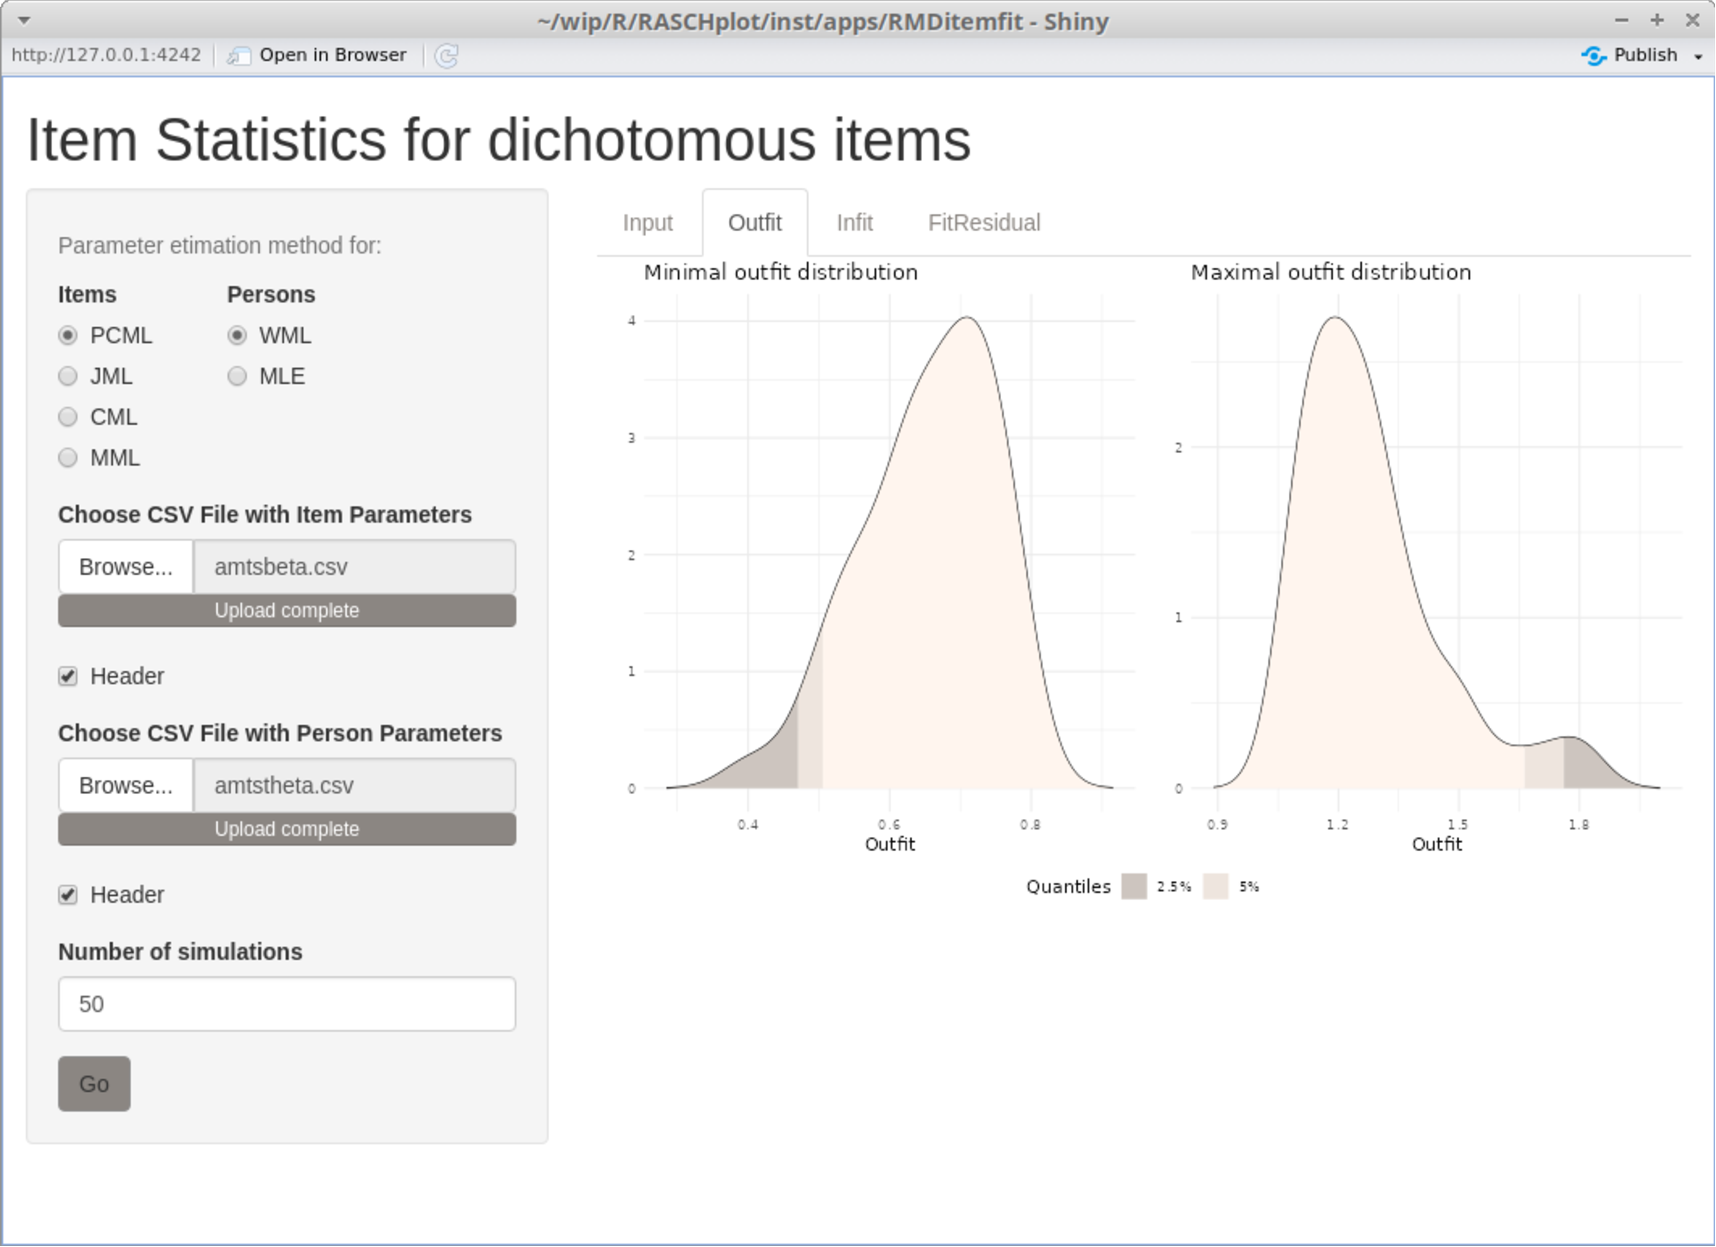
\includegraphics[width = .8\textwidth]{outfittab}
    \caption{Screenshot of the outfit item fit statistic visualisation page.}
    \label{fig:outfittab}
\end{figure}

